
% Prepared by Calvin Kent
%
% Assignment Template v19.02
%
%%% 20xx0x/MATHxxx/Crowdmark/Ax
%
\documentclass[12pt]{article} %
\usepackage{CKpreamble}
\usepackage{CKassignment}
\usepackage{tkz-euclide}
\usepackage{physunits}
\usepackage{physics}
\usepackage{lmodern}
\usepackage{microtype}
\usepackage{upgreek}
\usepackage[misc]{ifsym}


%%Title
\title{Functions Test 1}
\date{December 14, 2021}

%%% Maths and science packages

\usepackage{amsmath,amsthm,amssymb}
\usepackage{pgfplots}
	\usetikzlibrary{
		calc,
		patterns,
		positioning
	}
	\pgfplotsset{
		compat=1.16,
		samples=200,
		clip=false,
		my axis style/.style={
			axis x line=middle,
			axis y line=middle,
			legend pos=outer north east,
			axis line style={
				->,
			},
			legend style={
				font=\footnotesize
			},
			label style={
				font=\footnotesize
			},
			tick label style={
				font=\footnotesize
			},
			xlabel style={
				at={
					(ticklabel* cs:1)
				},
				anchor=west,
				font=\footnotesize,
			},
			ylabel style={
				at={
					(ticklabel* cs:1)
				},
				anchor=west,
				font=\footnotesize,
			},
			xlabel= $x$,
			ylabel=$\vec d (\m \tx{[East]})$
		},
	}
	\tikzset{
		>=stealth
	}

%%% Tables and figures packages

\usepackage{float}
\usepackage{caption}
	\captionsetup{
		format=plain,
		labelfont=bf,
		font=small,
		justification=centering
	}
	
%%% Numbers and sets

\newcommand{\E}{\mathrm{e}}

\newcommand{\tx}[1]{\text{#1}}

\begin{document}
    \pagenumbering{arabic}
    % Start of class settings ...
    \renewcommand*{\coursecode}{MCR3U Quiz} % Quiz Title
    \renewcommand*{\assgnnumber}{1} % Quiz number
    \renewcommand*{\submdate}{November, 2021} % renew the date
    \renewcommand*{\studentfname}{\textbf{Name:}} % Student first name
    \renewcommand*{\studentlname}{} % Student last name
    %\renewcommand*{\studentnum}{SNumber} % Student number

    \renewcommand\qedsymbol{$\blacksquare$}
    \setfigpath
    % End of class settings 
    \newgeometry{left=18mm, right=18mm, top=22mm, bottom=22mm} % page is set to default values
    \fancyhfoffset[L,O]{0pt} % header orientation fixed
    % End of class settings
    %%% Note to user:
    % CTRL + F <CHANGE ME:> (without the angular brackets) in CKpreamble to specify graphics paths accordingly.
    % The command \circled[]{} accepts one optional and one mandatory argument.
    % Optional argument is for the size of the circle and mandatory argument is for its contents.
    % \circled{A} produces circled A, with size drawn for letter A. \circled[TT]{A} produces circled A with size drawn for TT.
    % https://github.com/CalvinKent/My-LaTeX
    %%%
    % Crowdmark assignment start


    %%%%%%%%%%%%%%%%%%%%%%%%%%%%%%%%%%%%%%%%%%%%%%%%%%%%%%%%%%%%%%%%%%%%%%%%%%%%%%%%%%%%%%%%%%%%%%%%%%%%%%%%
    %%%%%%%%%%%%%%%%%                  PROBLEM IDEAS                  %%%%%%%%%%%%%%%%%%%%%%%%%%%%%%%%%%%%%%
    %%%%%                   ----------------------------------------                                %%%%%%%%

    % --> Do a hard tangent line problem

	\maketitle
	\section{Preamble}
	This is a test covering what we have learnt so far in lecture. Student's \emph{must show all work} to receive full marks.
	\section{Allowed Aids}
	The following aids are allowed on the Test
	\begin{itemize}
		\item Pencil, Pen, Eraser, Highlighter, Ruler, Protractor, Spare sheets of \textbf{blank} paper.
		\item Reference sheet \textbf{(Double sided paper preprepared by student)}
	\end{itemize}
	\section{Restrictions:}
  \begin{itemize}
		\item \textbf{NO} calculator's.
  \end{itemize}
  \section{Remarks:}
  \begin{itemize}
    \item $\mathbb N = \{1,2,3,4,5,\dots\} $.
    \item $\operatorname{rem}(x,y)$ is the remainder when you divide $x$ by $y$.
  \end{itemize}
	\section{Name and Date:}
	Print your name and todays date below;\\

	\begin{center}
	\noindent\begin{tabular}{ll}
		\makebox[3in]{\hrulefill} & \makebox[3in]{\hrulefill}\\
		Name & Date\\[8ex]% adds space between the two sets of signatures
	\end{tabular}
	\end{center}
	\newpage


\begin{qstn} % qnumber, qname, qpoints
  (10 marks) Answer the following True/False questions,
  \begin{enumerate}
    \item Let $\mathcal{R} = \{4,5,6,7,8\} $ and $\mathcal{H} = \emptyset $, then $\mathcal{R} + \mathcal{H} = \emptyset $.\\
      Circle the correct answer: \,\, \textbf{True} \,\,\,\,\,\, \textbf{False}

    \item Let $S = \{3,4,5\} $, then $S + S = S$.\\
      Circle the correct answer: \,\, \textbf{True} \,\,\,\,\,\, \textbf{False}

    \item $(\sqrt{4} + \pi) \in \Z$.\\
      Circle the correct answer: \,\, \textbf{True} \,\,\,\,\,\, \textbf{False}

    \item The vertex of 
      \[
        f(x) = 3\left( x + \pi \right)^2 - \sqrt{16}  
      \] is $(-\pi,-8)$.\\ 
      Circle the correct answer: \,\, \textbf{True} \,\,\,\,\,\, \textbf{False}

    \item The centre of the circle,
      \[
            (x-1)^2 + (y -2)^2 = 4
      \] is $(-1,-2)$.\\
      Circle the correct answer: \,\, \textbf{True} \,\,\,\,\,\, \textbf{False}

    \item The vertex of,
      \[
            f(x) = -\left( x - 3 \right)^2 - 4
      .\] represents a maximum.\\
      Circle the correct answer: \,\, \textbf{True} \,\,\,\,\,\, \textbf{False}
    \item The Domain and Range of,
      \[
              f(x) = -\frac{4}{2x + 1} + 8
    .\] is $\mathcal{D} = \{x \in \R \mid x \neq \frac{1}{2}\} $, $\mathcal{R} = \{y \in \R \mid y \neq 8\} $.\\
      Circle the correct answer: \,\, \textbf{True} \,\,\,\,\,\, \textbf{False}

    \item If $\mathcal{V} = \{v \in \mathbb N \mid v^2 = -1\}$, then $\mathcal{V}$ is the empty set.\\
      Circle the correct answer: \,\, \textbf{True} \,\,\,\,\,\, \textbf{False}

    \item The x-intercepts of $f(x) = x^2 -5x + 6$ are $x_1 = -2$ and $x_2 = -3$.\\
      Circle the correct answer: \,\, \textbf{True} \,\,\,\,\,\, \textbf{False}

    \item The vertex of $f(x) = x^2 + 6x + 5$ is $(-3,-4)$. \\
      Circle the correct answer: \,\, \textbf{True} \,\,\,\,\,\, \textbf{False}\\
      \textbf{Hint:} Save time by going from factored form to vertex\\
  \end{enumerate}
\end{qstn}

\newpage

\begin{qstn}
  (4 marks) Write down the elements of the following sets.\\
  (\textbf{Recall:} $\mathbb N = \{1,2,3,4,\dots\} $)
  \begin{enumerate}[label=(\alph*)]
    \item $\mathcal{T} = \{a \in \Z \mid 3 < a < 7\} $.
      \vspace*{5cm}

    \item $\mathcal{X} = \{x \in \mathbb N \mid x \neq 1 \} $.
      \vspace*{5cm}

    \item $\mathcal{Z} = \{y \in \mathbb Z \mid -3 \leq y \leq 0\} +  \{i \in \mathbb Z \mid -2 \leq i \leq 1\}$ \\
      \textbf{Hint:} Add the two sets first.
      \vspace*{5cm}

    \item $\mathcal{B} = \{x \in \mathbb N \mid \operatorname{rem}(x,2) = 0\} $.

  \end{enumerate}
\end{qstn}

\newpage

\begin{qstn}
  (8 marks) Determine the Domain and Range of the following functions,
  \begin{enumerate}[label=(\alph*)]
    \item $\mathcal{Y}(x) = -2\sqrt{5x - 10} - 8$.
      \vspace*{5cm}

    \item $x^2 + (y + 4)^2 = 16$.
      \vspace*{5cm}
    
    \item $\mathcal{L}(x) = -5\left|x + 1\right| - 3$.
      \vspace*{5cm}

    \item $\mathcal{E}(x) = -\frac{5}{2x - 10} + 5$.
  \end{enumerate}
\end{qstn}

\newpage

\begin{qstn}
 Lets define the following function,
  \begin{align*}
    f &\colon \R \to \R\\
    f(x) &= -x^2 + 4x + 3
  \end{align*}
  \begin{enumerate}[label=(\alph*)]
    \item (4 marks) Convert $f(x)$ into vertex form by completing the square.
      \vspace*{6cm}


    \item (3 marks) Sketch the function on the plot below. \textbf{(Label y-intercept and vertex)}
    \begin{center}
        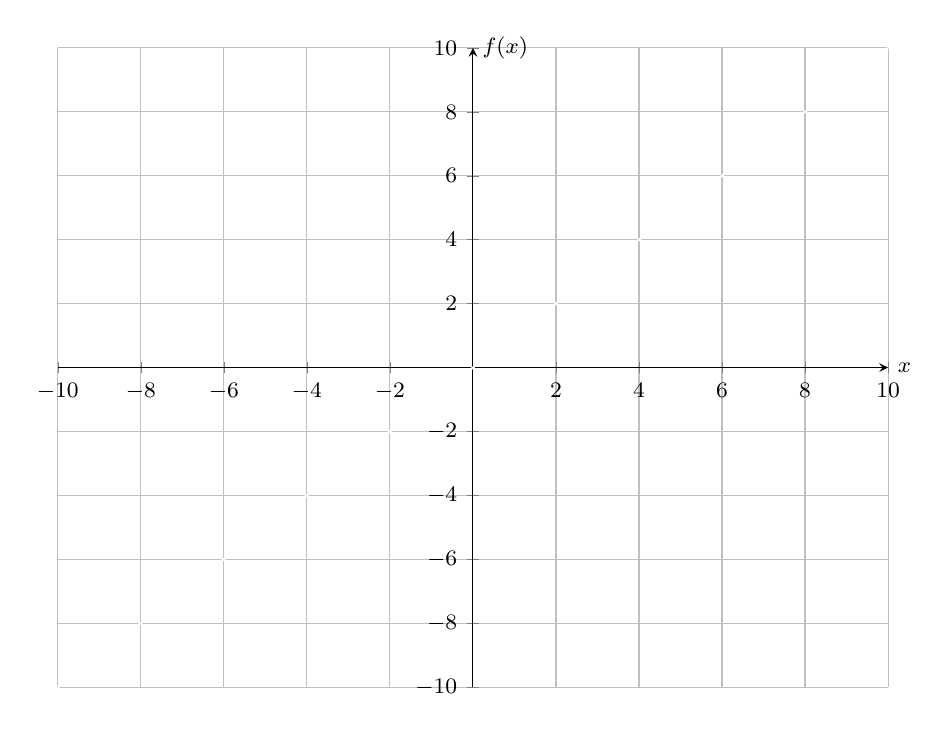
\begin{tikzpicture}
        \begin{axis}[
            my axis style,
            width=\textwidth,
            height=0.8\textwidth,
            ylabel=$f(x)$,
            grid
        ]
        
        \addplot[
            domain=-10:10,
            thick,
            white,
            -
        ]
        {x};

        \fill[
            black
        ];

        \end{axis}
        \end{tikzpicture}
    \end{center}
  \end{enumerate}
\end{qstn}

\begin{qstn}
  (2 marks) We call a function \emph{idempotent} if $f(f(x)) = f(x)$. Is the function \\
  $f(x) = x$ \emph{idempotent}? Justify your answer.
\end{qstn}
\vspace*{4cm}

\begin{qstn}
  (7 marks) Factor the following quadratic functions,
  \begin{enumerate}[label=(\alph*)]
    \item $f\left( x \right) = -x ^2 +9x -20$.
      \vspace*{5cm}

    \item $f(x) = 4x^2 - 1$.
      \vspace*{5cm}

    \item $f\left( x \right) = 2x^2 - 4x - 16$.\\
      \textbf{Hint:} This \emph{can} be factored simply.
  \end{enumerate}
\end{qstn}

\newpage

\begin{qstn}
  (6 marks) Let $g(x) = 5x^2 + 14x - 3$,
  \begin{enumerate}[label=(\alph*)]
    \item How many solutions will $g(x)$ have? (\textbf{Note: }$14^2 = 196$)
      \vspace*{3cm}

    \item Factor $g(x)$.
      \vspace*{7cm}

  \end{enumerate}
\end{qstn}

\begin{qstn}
  (6 marks) Let $T(x) = -\frac{1}{2}(2x - 22)(x + 1)$. Convert $T(x)$ into vertex form.
\end{qstn}

\newpage

\begin{qstn}
  (6 marks) A function is \emph{nilpotent} if there exists some number $t$ such that \\
  $f(f(t)) = 0$. Let  $T(x) = x^2 - 1$.
  \begin{enumerate}[label=(\alph*)]
    \item Determine $T(T(1))$.
      \vspace*{4cm}

    \item Determine $T(T(0))$.
      \vspace*{4cm}

    \item Is $T(x)$ \emph{nilpotent}? Justify your answer.
      \vspace*{2cm}

  \end{enumerate}
\end{qstn}

\begin{qstn}
  (6 marks) Let $f(x) = x - 1$ and $g(x) = x + 1$. We call $f$ and $g$ \emph{mutual inverses} of each other if \textbf{both} of the following conditions
  hold,
  \begin{itemize}
    \item For every number $b$,  $f(g(b)) = b$.
    \item For every number $a$,  $g(f(a)) = a$.
  \end{itemize}

  \begin{enumerate}[label=(\alph*)]
    \item Determine $f(g(1))$.
      \newpage

    \item Determine $g(f(2))$.
      \vspace*{4cm}

    \item Based on your answers from part (a) and (b), do you think $f$ and $g$ are inverses of each other?
      \vspace*{4cm}

  \end{enumerate}
\end{qstn}

\begin{qstn}
  (6 marks) Let $S = \{x \in \R \mid 8x^2 + 2x - 3 = 0\}$. Write down the elements of $S$.\\
  \textbf{Hint: }Try factoring first.
\end{qstn}


\end{document}






























